\documentclass[a4paper, 10pt]{article}
    \usepackage[subpreambles=true]{standalone}
    \usepackage[english, american, british]{babel}
    \usepackage[utf8]{inputenc}
    \usepackage[T1]{fontenc}
    \usepackage{hyphenat}
    \hyphenation{Mathe-matik wieder-gewinnen}
    \usepackage{amsmath}
    \usepackage{import}
    \usepackage{tabularx}
    \usepackage{graphicx}
    \usepackage{makecell}
    \usepackage{verbatim}
    \usepackage[margin=1cm ]{geometry}

    \title{Einführung in die Softwaretechnik 2018 \\ Sheet 06}
    \author{Maximilian Frühauf}

\begin{document}
\maketitle
\begin{enumerate}
    \item You are designing the access control mechanism for a web-based retail store. 
    Customers browse product information, update their profile, and purchase products. 
    Suppliers can add new products, update product information, and create, process, and examine orders. 
    The store administrator sets the retail prices, makes tailored offers to customers based on their purchasing profiles, 
    and provides marketing services. You have to deal with four actors: StoreAdministrator, Supplier, 
    registered Customer, and unregistered WebUser. Design an access control mechanism for all actors. 
    Customers are already registered. Suppliers need to be registered by the StoreAdministrator. 
    Unregistered web users can only get information about the product and can register by creating the customer info.

    \vspace{0.5cm}

    \begin{table}[h!]
        \centering
        \begin{tabular}{ m{2cm} || c | c | c | c | c  }
            \hline
            Actors / Objects & Product & Order & Offer & Profile & Marketing \\
            \hline
            \hline
            Store Administrator & \makecell{set retail Price} & & \makecell{<<create>> \\ make offer} & \makecell{ read purchase info* \\ <<create>> \\ register Supplier} & provide marketing services \\
            \hline 
            Supplier & \makecell{<<create>> \\ add product \\ update product info } & \makecell{<<create>> \\ create order \\ process \\ examine } &  &  & \\
            \hline 
            registered Customer & \makecell{browse product information  \\ purchase product} &  & & update profile & \\
            \hline 
            unregistered WebUser & browse product information &  && \makecell{<<create>> \\ register user} &\\ 
        \end{tabular}
    \end{table}

    * As the StoreAdministrator needs to be able to make offers based on a Customers purchasing history 
    ha has to able to read the data from the profile method. Therefore this extra functionality is added.
    \item
    Given the following sentences, which inheritance mechanisms (specification or implementation inheritance) would be appropriate?
    \begin{itemize}
        \item A Rectangle class inherits from a Polygon class.
        \item A Set class inherits from an existing BinaryTree class.
        \item A Set class inherits from a Bag class (a Bag is defined as an unordered collection).
        \item A Player class inherits from a User class.
    \end{itemize}
    \vspace{0.5cm}


    \begin{itemize}
        \item Rectangle inherits form Polygon

        As Polygon is more abstract than the Rectangle specification inheritance is used.
        This is the case because a Rectangle is polygon but only the specification of that functionality is reused.
        \item Set inherits from BinaryTree 

        Here implementation inheritance is used as BinaryTree is a concrete implementation of an Algorithm
        and set reusing this provided functionality.
        \item  Set inherits from Bag 

        Here specification inheritance is used as bag is an abstract definition of an unordered collection 
        and Set implements it. Therefore only the specified functionality is reused.
        \item Player inherits form User 

        Here specification is used as User is a more abstract concept than Player. Because of this the 
        functionality specified in the User class is implemented in the Player.
    \end{itemize}


    \item Consider a workflow system supporting software developers. 
    The system enables managers to model the process the developers should follow in 
    terms of processes and work products. The manager assigns specific processes to each developer and sets deadlines 
    for the delivery of each work product. The system supports several types of work products: 
    formatted text, pictures, and URLs. The manager, while editing the workflow, can dynamically set each 
    work product’s type at run-time. 
    Assuming one of your design goals is to design the system so that more work product types can be added in the future, 
    which design pattern would you use to represent work products? 
    Justify your choice and model this design pattern using a UML class diagram.
    \vspace{0.5cm}

    \begin{center}
        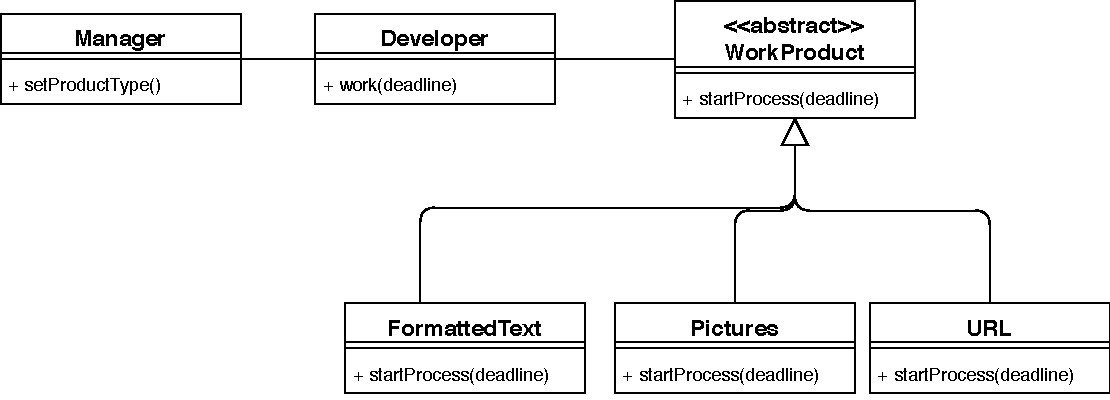
\includegraphics[width=15cm]{Task03.pdf}
    \end{center}

    This system is realized with the bridge patten as the concrete implementation of a 
    work product needs to be chosen at runtime. The choice of this pattern is reinforced as 
    the list of possible WorkProduct Types needs to be easily extensible.

    Therefore once a Manager assigns a WorkProduct via the \verb+work(deadline)+ method with a specified deadline,
    the Corresponding WorkProduct implementation is chosen. As all of them have the \verb+startProcess(deadline)+ method 
    a specification with an interface  is done.

    \item
    A server offers a method to perform an encryption. 
    A variety of clients can use this method. At run-time, 
    the server application selects the AES or DES encryption algorithm. 
    AES supports a variety of key lengths with 128, 192, to 256-bit, whereas DES only supports 56-bit keys. 
    The server has to deal with clients that require backward compatibility and clients that require high security. 
    Draw a UML class diagram depicting the classes and methods, and explain your model.
    \vspace{0.5cm}

    \begin{center}
        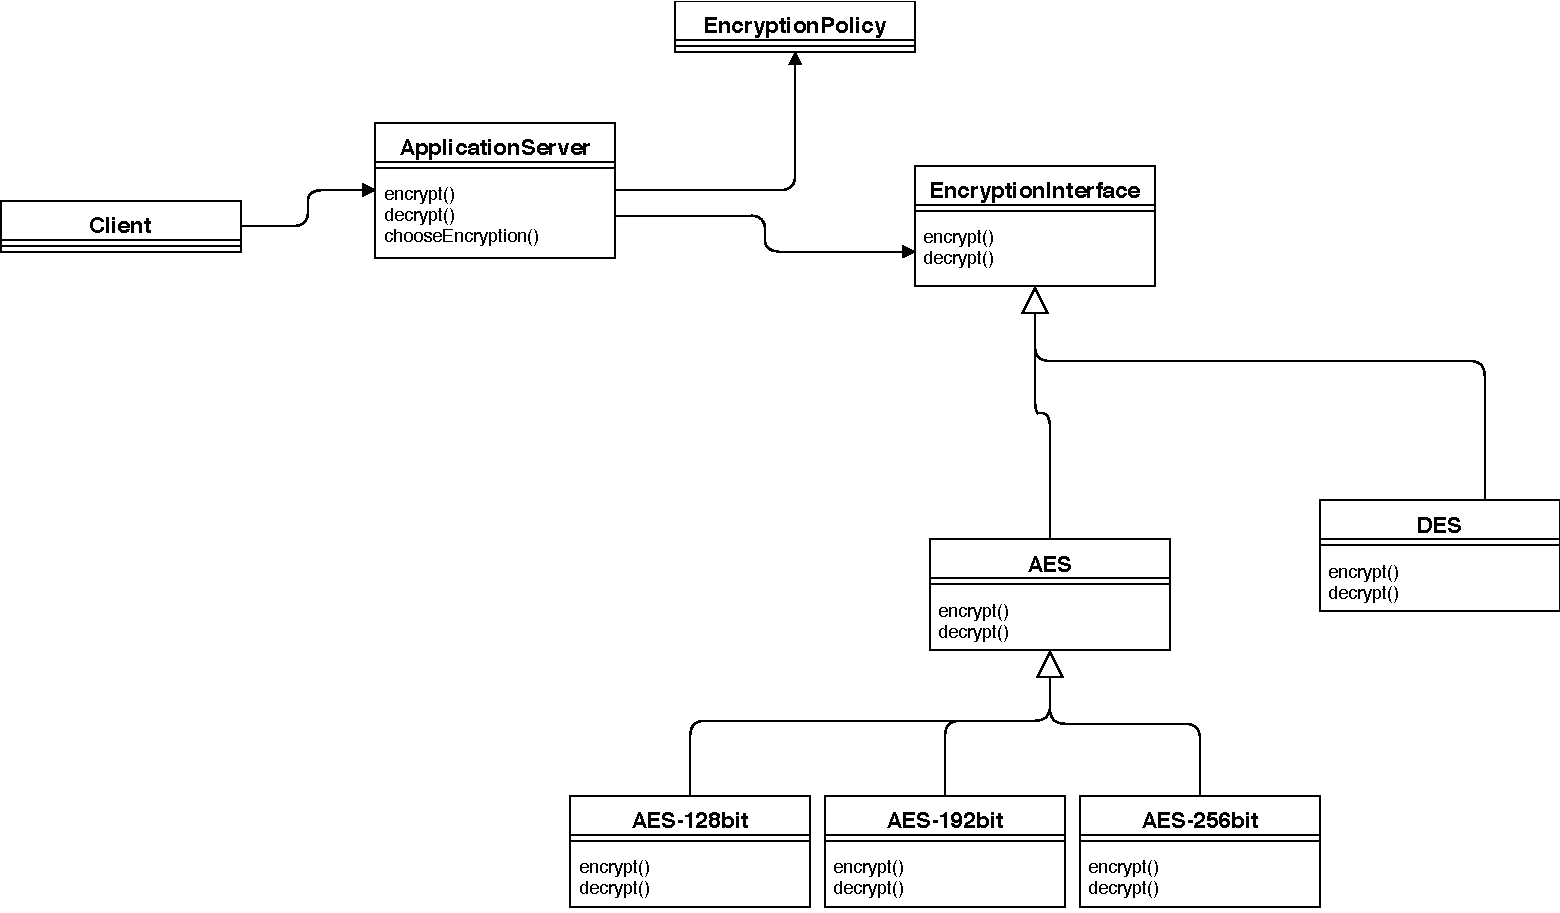
\includegraphics[width=15cm]{Task04.pdf}
    \end{center}

    When a connection is initiated the Client connects to the application server and 
    an encryption strength is decided upon by the \verb+chooseEncryption()+ Method. It uses 
    the encryption policy to decide upon the right encryption to use at runtime. This is based on the 
    capabilities of the client. If it is a legacy one DES is used, otherwise AES.

    Once the encryption type (AES / DES) is chosen the strongest possible cypher length is chosen. 
    Then the corresponding object is instantiated and used to encrypt the message. The result is then send back 
    to the client. Decryption is handled the same way except that the encryption policy always choses the encryption type
    of the encrypted message to be able to get back at the original message.
    \item
    Explain the differences between inheritance and delegation. 
    \vspace{0.5cm}

    When utilizing inheritance an existing class is extended and functionality can be added or modified. 
    This allows the reuse of functionality implemented in the super class. This feature of most programming languages 
    is straightforward to use and makes it easy to implement new functionality in existing classes.
    However during this process the public methods of the parent class are exposed on each subclass and 
    changes in a parent class also affect all children.

    Delegation mediates access to an object via a Receiver. The Clients class it are then passed on to
    the Delegate and modified if necessary.
    This process makes sure that it is impossible to for the client to misuse the features of the Delegate object.
    The pattern also allows the exchange of any object (Receiver or Delegate) as long as they are of the same type.
    This flexibility comes at the cost of efficiency as objects are encapsulated in this pattern. 

\end{enumerate}
\end{document}